\documentclass{article}
\usepackage{graphicx}
\usepackage{multicol} % use to multiple column in itemize
\usepackage{float}
\usepackage{setspace}
\usepackage{hyperref}
\usepackage[draft]{todonotes}
\usepackage{marginnote}
\setlength{\parskip}{0.5em}

\begin{document}

\title{Determining features}
% \author{Cong Cuong PHAM}

\maketitle

\begin{abstract}
This document introduces some fundamental notions of Determining features, Feature importance and Determining features.
\end{abstract}

\subsection{Determining features}
\par \todo[size=\footnotesize]{collecting data as well as choosing features are important} With a challenge in mind you want to solve, you know that you need to collect a lot of samples along with features that describe them. This is the prerequisite for machine learning. You now also know these features can be continuous numeric values, or they can be categorical. But how exactly should you go about choosing features? And what's more important to focus on—adding additional features or collecting more samples?

\par \todo[size=\footnotesize]{The answerm it depends.}These are reasonable questions everyone has when they start amassing the data they need to solve an issue. The answer is, it depends. Just as in the example of Angie \& Craig's lists mentioned in the Machine Learning section, your own intuition about the problem being tackled should really be the driving force behind what data you collect. The only unbreakable rule is that you {\bf{need to ensure you collect as many features and samples as you possibly can}}.

\par If you ever become unsure which one of the two you should focus on more, concentrate on collecting more samples. A least during collection, try to make sure you have more samples than features because some machine learning algorithms won't work well if that isn't the case. This is also known as the curse of dimensionality. At its core, many algorithms are implemented as matrix operations, and without a greater than or equal number of samples to features, a fully-formed system of independent equations cannot be made. You can always create {\it{more}} features based off of your existing ones. But creating {\it{pseudo-samples}}, while not impossible, might be a bit more difficult \todo[size=\footnotesize]{Ensure that number of samples is greater than number of features.}.

\begin{figure}[H]
\centering
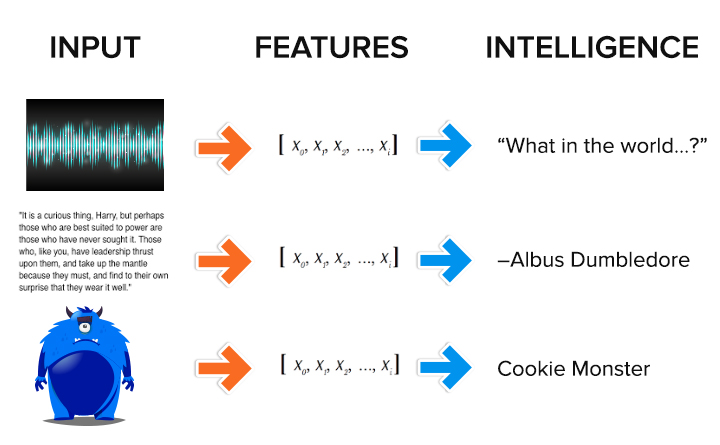
\includegraphics[width=.8\linewidth]{pic/determining-features.png}
\end{figure}
  
\subsection{Feature importance}
\par After coming up with a bunch of features to describe your data, you might be tempted to investigate which of them deliver the most bang for their buck. Try not to fall into this trap by making too many assumptions about which features are truly relevant! There will be plenty of time and better tools for doing that later in the data analysis process. While out collecting, time spent deliberating whether you should move forward with a particular feature is time not spent adding more samples into your dataset! What more, if you were already aware of a single {\it{golden feature}} \marginpar{{\it{golden feature}}} that completely resolved your challenge and answered the question you had in mind, rather than approaching the problem through data analysis and machine learning, you could probably directly engineer a solution around that single attribute.

\par Data-driven problems can reach a level of complexity where even with your expertise in the problem's domain, you still are only vaguely able to derive a few noisy features that do a bad job of describing the relationship you hope to model. Such {\it{sub-par features}} might only partially help answer your question by providing marginal information, but do not throw them away. Instead, use them as your feature set

\par Data-driven problems can reach a level of complexity where even with your expertise in the problem's domain, you still are only vaguely able to derive a few noisy features that do a bad job of describing the relationship you hope to model. Such {\it{sub-par features}} might only partially help answer your question by providing marginal information, but do not throw them away. Instead, use them as your feature set.

\par Let's say you want to get your pet iguana Joey a special treat for his birthday. Joey is super picky in his eating habits. You know he generally likes dark, green, leafy vegetables like kale and mustard greens; but occasionally he {\it{violently}} rejects them. Joey can't communicate to you why he sometimes like's them or other times doesn't. But being a data driven person, you've long since theorized there must be a method to the madness, and have been keeping some stats on all the food you've ever given him. Of particular interest are two features: fiber, and antioxidant content.

\par Individually, these features seem like poor indicators of Joey's preference of food. It looks like he likes some low-fibrous greens, but he also likes greens that are packed with them. What gives? By combining these two features, you realize there truly is a succinct way of correctly identifying veggies Joey likes, each time every time (the blue plots)!

\begin{figure}[H]
\centering
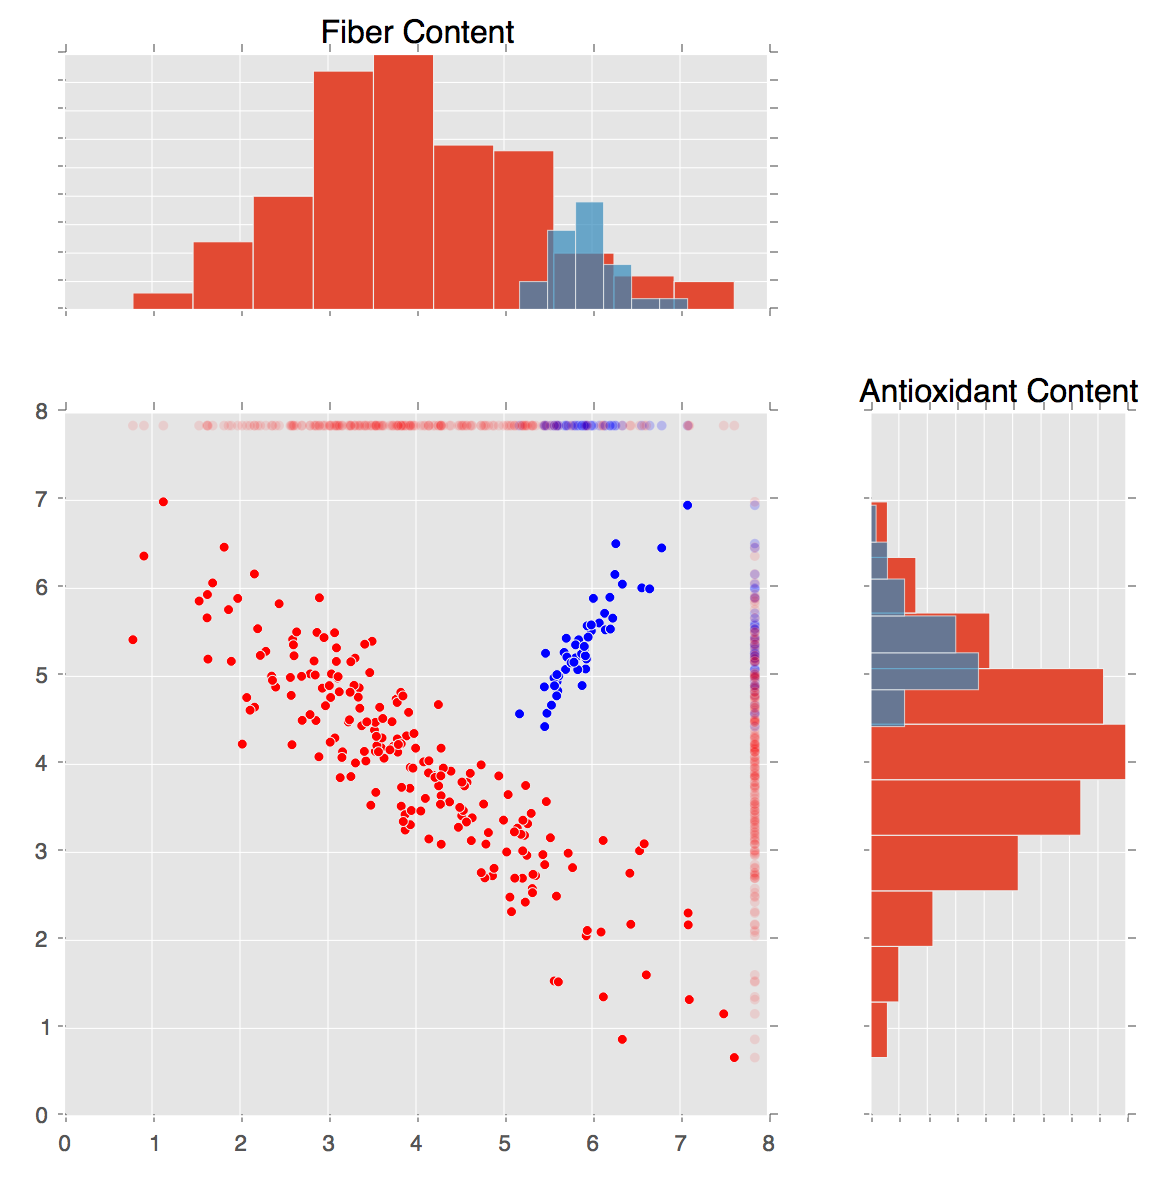
\includegraphics[width=.8\linewidth]{pic/feature-importance.png}
\end{figure}

\subsection{General guidelines}
\par Everything just mentioned only applies if you're given the creative freedom to go out and collect your own data! If you are given data to work with, all you're really able to do is come up with nifty ideas for combining existing features to form new and beneficial derivatives.

\par Your machine learning goal should be to train your algorithms instead of hard coding them. When it comes to deriving features, approach them the same way. Let your expertise and intuition guide you, by brainstorming what data you would need to collect to meet the goals of your analysis. Think of your machine learning models as if they were small children who have absolutely no knowledge except what you train them with; what information would they need to know to make the right decisions?

\par There are no hard and fast rules when it comes to thinking up good features for your samples; but a rule does exist about what to avoid: garbage. If you collect details about your samples that you know is statistically irrelevant to the domain of the problem you're trying to solve, you'll only be wasting your time and eroding the accuracy of your analysis.{\it{Garbage in, garbage out}}.\marginpar{\it{Garbage in, garbage out}}

\par If you're trying to have machine learning model a regression relationship between various car features (MPG, comfort level, current mileage, year manufactured, \# cylinders, has turbo, etc.) and car costs, introducing features like car color or air freshener scent probably won't do you that much good. In order for machine learning to do its job of finding a relationship in your data, {\it{in your data, a relationship must exist}}.

\begin{flushright}
    source: \href{https://courses.edx.org/courses/course-v1:Microsoft+DAT210x+6T2016/courseware/12621a4064aa4d92874a9d8a953734c5/dfc5af6b20e548b4a62b59b73d71d9bd/}{course.edx.org}  
\end{flushright}

\end{document}